\documentclass[12pt,letterpaper]{article}
\usepackage{graphicx,textcomp}
\usepackage{natbib}
\usepackage{setspace}
\usepackage{fullpage}
\usepackage{color}
\usepackage[reqno]{amsmath}
\usepackage{amsthm}
\usepackage{fancyvrb}
\usepackage{amssymb,enumerate}
\usepackage[all]{xy}
\usepackage{endnotes}
\usepackage{lscape}
\newtheorem{com}{Comment}
\usepackage{float}
\usepackage{hyperref}
\newtheorem{lem} {Lemma}
\newtheorem{prop}{Proposition}
\newtheorem{thm}{Theorem}
\newtheorem{defn}{Definition}
\newtheorem{cor}{Corollary}
\newtheorem{obs}{Observation}
\usepackage[compact]{titlesec}
\usepackage{dcolumn}
\usepackage{tikz}
\usetikzlibrary{arrows}
\usepackage{multirow}
\usepackage{xcolor}
\newcolumntype{.}{D{.}{.}{-1}}
\newcolumntype{d}[1]{D{.}{.}{#1}}
\definecolor{light-gray}{gray}{0.65}
\usepackage{url}
\usepackage{listings}
\usepackage{color}

\definecolor{codegreen}{rgb}{0,0.6,0}
\definecolor{codegray}{rgb}{0.5,0.5,0.5}
\definecolor{codepurple}{rgb}{0.58,0,0.82}
\definecolor{backcolour}{rgb}{0.95,0.95,0.92}

\lstdefinestyle{mystyle}{
	backgroundcolor=\color{backcolour},   
	commentstyle=\color{codegreen},
	keywordstyle=\color{magenta},
	numberstyle=\tiny\color{codegray},
	stringstyle=\color{codepurple},
	basicstyle=\footnotesize,
	breakatwhitespace=false,         
	breaklines=true,                 
	captionpos=b,                    
	keepspaces=true,                 
	numbers=left,                    
	numbersep=5pt,                  
	showspaces=false,                
	showstringspaces=false,
	showtabs=false,                  
	tabsize=2
}
\lstset{style=mystyle}
\newcommand{\Sref}[1]{Section~\ref{#1}}
\newtheorem{hyp}{Hypothesis}

\title{Problem Set 3}
\date{Due: November 11, 2024}
\author{Applied Stats/Quant Methods 1}


\begin{document}
	\maketitle
	\section*{Instructions}
	\begin{itemize}
		\item Please show your work! You may lose points by simply writing in the answer. If the problem requires you to execute commands in \texttt{R}, please include the code you used to get your answers. Please also include the \texttt{.R} file that contains your code. If you are not sure if work needs to be shown for a particular problem, please ask.
	\item Your homework should be submitted electronically on GitHub.
	\item This problem set is due before 23:59 on Sunday November 11, 2024. No late assignments will be accepted.

	\end{itemize}

		\vspace{.25cm}
	
\noindent In this problem set, you will run several regressions and create an add variable plot (see the lecture slides) in \texttt{R} using the \texttt{incumbents\_subset.csv} dataset. Include all of your code.

	\vspace{.5cm}
\section*{Question 1}
\vspace{.25cm}
\noindent We are interested in knowing how the difference in campaign spending between incumbent and challenger affects the incumbent's vote share. 
	\begin{enumerate}
		\item Run a regression where the outcome variable is \texttt{voteshare} and the explanatory variable is \texttt{difflog}.	
		\lstinputlisting[language=R, firstline=38, lastline=39]{my_answers_RJ.C.R}
		\begin{verbatim}
		Call:
		lm(formula = voteshare ~ difflog, data = df)
		
		Residuals:
		   Min     1Q       Median    3Q       Max 
		-0.26832 -0.05345  -0.00377  0.04780  0.32749 
		
		Coefficients:
		           Estimate Std. Error     t value   Pr(>|t|)    
		(Intercept) 0.579031     0.002251   257.19   <2e-16 ***
		difflog     0.041666     0.000968   43.04    <2e-16 ***
		---
		Signif. codes:  0 ‘***’ 0.001 ‘**’ 0.01 ‘*’ 0.05 ‘.’ 0.1 ‘ ’ 1
		
		Residual standard error: 0.07867 on 3191 degrees of freedom
		Multiple R-squared:  0.3673,	Adjusted R-squared:  0.3671 
		F-statistic:  1853 on 1 and 3191 DF,  p-value: < 2.2e-16
		\end{verbatim}
		\begin{verbatim}
			Data analysis:
			The residual standard error is 0.07867, which measures the average difference 
			between observed values and model predictions. The degree of freedom is 3191. 
			The coefficient of determination is 0.3673. This value represents the proportion 
			of variability explained by the model, meaning that the model explained 36.73% 
			of the variability. The adjusted coefficient of determination is 0.3671, 
			and the R-squared value has been adjusted to avoid overfitting due to 
			the addition of irrelevant variables. The F-statistic is 1853, 
			which is used to test whether all coefficients in the model are significantly 
			different from 0. The F-statistic of 1853 is very high, 
			indicating that the model is significant. The degrees of freedom of 
			the F-statistic are 1 and 3191. The p-value of the F-statistic is<2.2e-16, 
			indicating that the F-statistic is significant and the model has at least one 
			coefficient significantly different from 0.
		\end{verbatim}
		\vspace{0.005cm}
		\item Make a scatterplot of the two variables and add the regression line. 	
		\lstinputlisting[language=R, firstline=40, lastline=45]{my_answers_RJ.C.R}
		\begin{enumerate}
			\item[]
			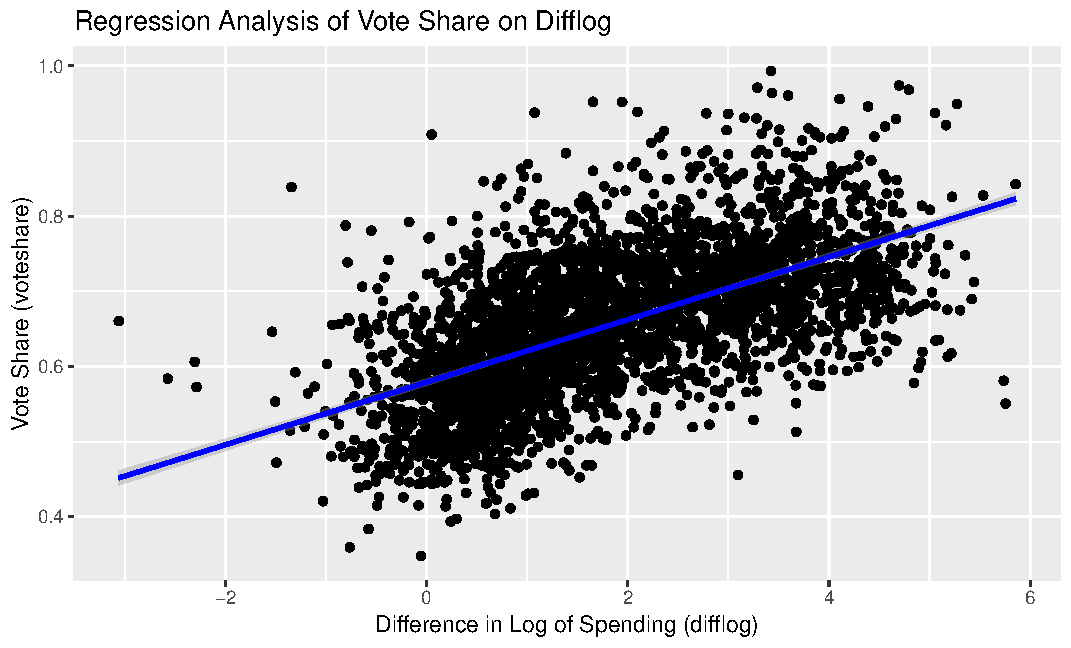
\includegraphics[width=.70\textwidth]{my_answers_question1.1_plot.pdf}
		\end{enumerate}
		\vspace{0cm}
		\item Save the residuals of the model in a separate object.
		\lstinputlisting[language=R, firstline=46, lastline=48]{my_answers_RJ.C.R}
		\begin{verbatim}
		View the first few data items:
	               1              2             3     
             -0.0004227622 -0.0316840149 -0.0045514943
	               4              5             6 
              0.0386688767  0.0355287965  0.0322832521 
		\end{verbatim}
		\begin{verbatim}
			Use a scatter plot to view the distribution of residuals
		\end{verbatim}
		\begin{enumerate}
			\item[]
			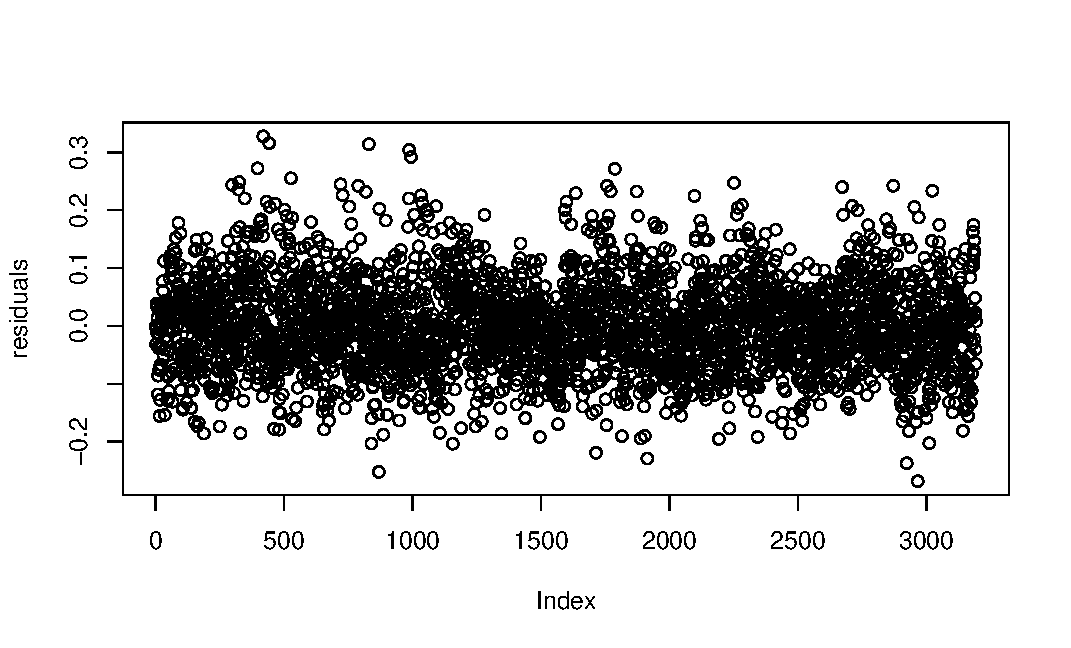
\includegraphics[width=.70\textwidth]{my_answers_question1.3_plot.pdf}
		\end{enumerate}
		\vspace{7cm}
		\item Write the prediction equation.
		\lstinputlisting[language=R, firstline=49, lastline=52]{my_answers_RJ.C.R}
		\begin{verbatim}
			the prediction equation:
			   voteshare = 0.579030710920674  +  0.0416663238227399 * difflog
		\end{verbatim}
	\end{enumerate}
	
\newpage

\section*{Question 2}
\noindent We are interested in knowing how the difference between incumbent and challenger's spending and the vote share of the presidential candidate of the incumbent's party are related.	\vspace{.25cm}
	\begin{enumerate}
		\item Run a regression where the outcome variable is \texttt{presvote} and the explanatory variable is \texttt{difflog}.	
		\lstinputlisting[language=R, firstline=55, lastline=56]{my_answers_RJ.C.R}
		\begin{verbatim}
			Call:
			lm(formula = presvote ~ difflog, data = df)
			
			Residuals:
			   Min       1Q     Median      3Q      Max 
			-0.32196 -0.07407  -0.00102   0.07151  0.42743 
			
			Coefficients:
			           Estimate Std.   Error    t value   Pr(>|t|)    
			(Intercept) 0.507583     0.003161   160.60   <2e-16 ***
			difflog     0.023837     0.001359   17.54   <2e-16 ***
			---
			Signif. codes:  0 ‘***’ 0.001 ‘**’ 0.01 ‘*’ 0.05 ‘.’ 0.1 ‘ ’ 1
			
			Residual standard error: 0.1104 on 3191 degrees of freedom
			Multiple R-squared:  0.08795,	Adjusted R-squared:  0.08767 
			F-statistic: 307.7 on 1 and 3191 DF,  p-value: < 2.2e-16
		\end{verbatim}
		\begin{verbatim}
			Data analysis:
			Residual analysis shows that the minimum residual is -0.32196, 
			the first quartile is -0.07407, the median is -0.00102, 
			the third and fourth quartiles are 0.07151, and the maximum residual is 0.42743. 
			This indicates that the residuals are distributed within a certain range and 
			there are no obvious outliers. The intercept is 0.507583, the standard error is 
			0.003161, the t-value is 160.60, and the p-value is less than 2e-16. 
			This means that the intercept is statistically significant. The slope is 0.023837,
			the standard error is 0.001359, the t-value is 17.54, and the p-value is less 
			than 2e-16. This indicates a significant positive correlation between difflog 
			and presvote.The residual standard error is 0.1104, based on 3191 degrees of 
			freedom. The coefficient of determination is 0.08795, and the adjusted 
			coefficient of determination is 0.08767. This indicates that difflog can explain 
			approximately 8.795% of the presvote variation. The F-statistic is 307.7, 
			based on 1 model degree of freedom and 3191 error degrees of freedom, 
			with a p-value less than 2.2e-16. This indicates that the overall model is 
			statistically significant.
			
			Conclusion:
			For every unit increase in difflog, the average increase in votes is 0.023837 
			units. The model is statistically significant, but its explanatory power is 
			limited, only explaining about 8.795% of the presvote variation. These results 
			indicate that although difflog has a significant impact on pre voting, 
			there may be other factors that are also affecting pre voting. 
			Further analysis may require consideration of more explanatory variables.
		\end{verbatim}
		\vspace{1cm}
		\item Make a scatterplot of the two variables and add the regression line. 	
		\lstinputlisting[language=R, firstline=57, lastline=62]{my_answers_RJ.C.R}
		\begin{enumerate}
			\item[]
			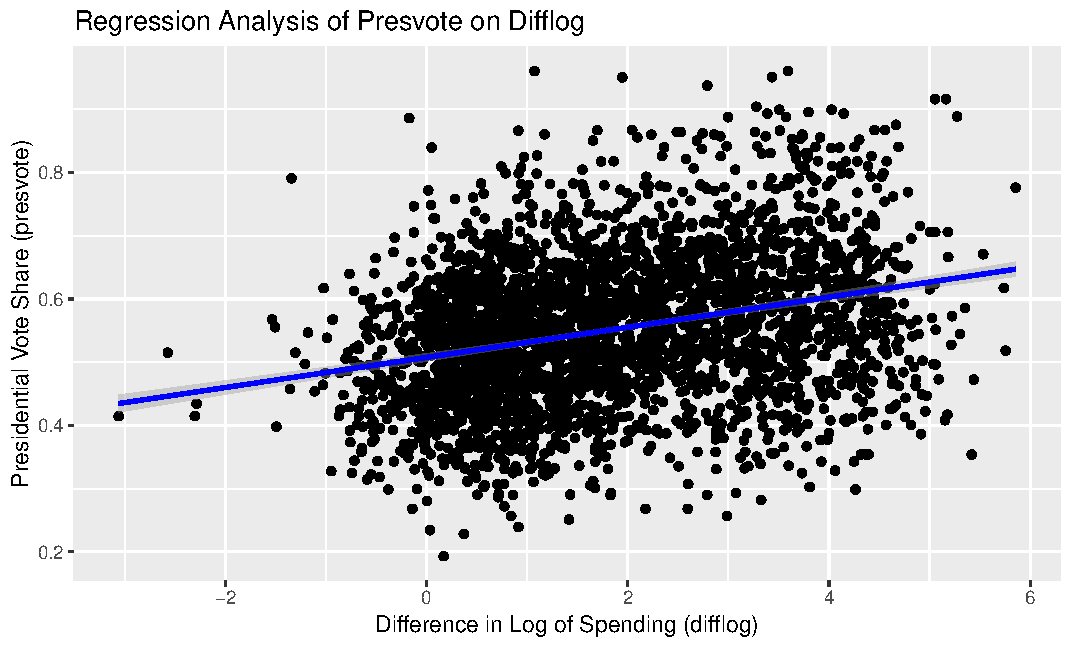
\includegraphics[width=.70\textwidth]{my_answers_question2.2_plot.pdf}
		\end{enumerate}
		\vspace{5cm}
		\item Save the residuals of the model in a separate object.
		\lstinputlisting[language=R, firstline=63, lastline=65]{my_answers_RJ.C.R}
		\begin{verbatim}
			View the first few data items:
			     1            2            3
			0.005605594  0.037578519 -0.053134788            
			     4            5            6 
		   -0.052993694 -0.045842994  0.074339701  
		\end{verbatim}
		\begin{verbatim}
			Use a scatter plot to view the distribution of residuals
		\end{verbatim}
		\begin{enumerate}
			\item[]
			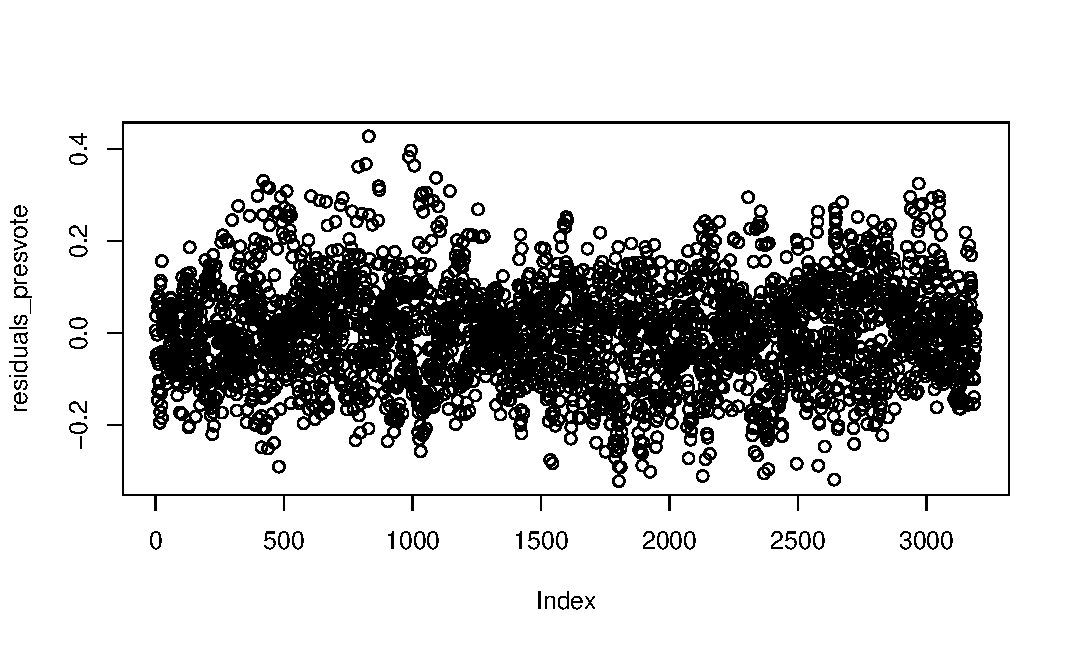
\includegraphics[width=.70\textwidth]{my_answers_question2.3_plot.pdf}
		\end{enumerate}
		\vspace{1cm}
		\item Write the prediction equation.
		\lstinputlisting[language=R, firstline=66, lastline=69]{my_answers_RJ.C.R}
		\begin{verbatim}
			the prediction equation:
			presvote = 0.507583328405015  +  0.023837233841334 * difflog
		\end{verbatim}
	\end{enumerate}
	
	\newpage	
\section*{Question 3}

\noindent We are interested in knowing how the vote share of the presidential candidate of the incumbent's party is associated with the incumbent's electoral success.
	\vspace{.25cm}
	\begin{enumerate}
		\item Run a regression where the outcome variable is \texttt{voteshare} and the explanatory variable is \texttt{presvote}.
		\lstinputlisting[language=R, firstline=72, lastline=73]{my_answers_RJ.C.R}
		\begin{verbatim}
			Call:
			lm(formula = voteshare ~ presvote, data = df)
			
			Residuals:
			   Min       1Q     Median     3Q      Max 
			-0.27330 -0.05888  0.00394  0.06148  0.41365 
			
			Coefficients:
			           Estimate Std. Error     t value   Pr(>|t|)    
			(Intercept) 0.441330     0.007599   58.08    <2e-16 ***
			presvote    0.388018     0.013493   28.76    <2e-16 ***
			---
			Signif. codes:  0 ‘***’ 0.001 ‘**’ 0.01 ‘*’ 0.05 ‘.’ 0.1 ‘ ’ 1
			
			Residual standard error: 0.08815 on 3191 degrees of freedom
			Multiple R-squared:  0.2058,	Adjusted R-squared:  0.2056 
			F-statistic:   827 on 1 and 3191 DF,  p-value: < 2.2e-16
		\end{verbatim}
		\begin{verbatim}
		Data analysis:
		Residual analysis shows that the minimum residual is -0.27330, the first quartile 
		is -0.05888, the median is 0.00394, the third and fourth quartiles 
		are 0.06148, and the maximum residual is 0.41365. This indicates that 
		the residuals are distributed within a certain range and there are no 
		obvious outliers. The intercept is 0.441330, the standard error is 
		0.007599, the t-value is 58.08, and the p-value is less than 2e-16. 
		This means that the intercept is statistically significant. Presvote: 
		0.388018, standard error of 0.013493, t-value of 28.76, p-value less 
		than 2e-16. This indicates a significant positive correlation between 
		presvote and vote share.
		The residual standard error is 0.08815, based on 3191 degrees of 
		freedom. The coefficient of determination is 0.2058, and the adjusted 
		coefficient of determination is 0.2056. This indicates that presvote 
		can explain approximately 20.58% of the variability in voteshare. The 
		F-statistic is 827, based on 1 model degree of freedom and 3191 error 
		degrees of freedom, with a p-value less than 2.2e-16. This indicates 
		that the overall model is statistically significant.
		
		Conclusion:
		For every additional unit of presvote, the average increase in voters 
		is 0.388018 units.
		The model is statistically significant and explains approximately 
		20.58% of the variance in vote share, indicating that presvote is a 
		useful variable for predicting vote share. These results indicate a 
		significant positive correlation between the voting share in the 
		presidential election and the voting share in the House of 
		Representatives election. However, it should be noted that although 
		the correlation is significant, the explanatory power of the model is 
		limited and can only explain a portion of the variation in voting 
		shares. This indicates that there are other factors also affecting 
		the voting share.
		\end{verbatim}
		\vspace{0cm}
		\item Make a scatterplot of the two variables and add the regression line. 
		\lstinputlisting[language=R, firstline=74, lastline=79]{my_answers_RJ.C.R}
		\begin{enumerate}
			\item[]
			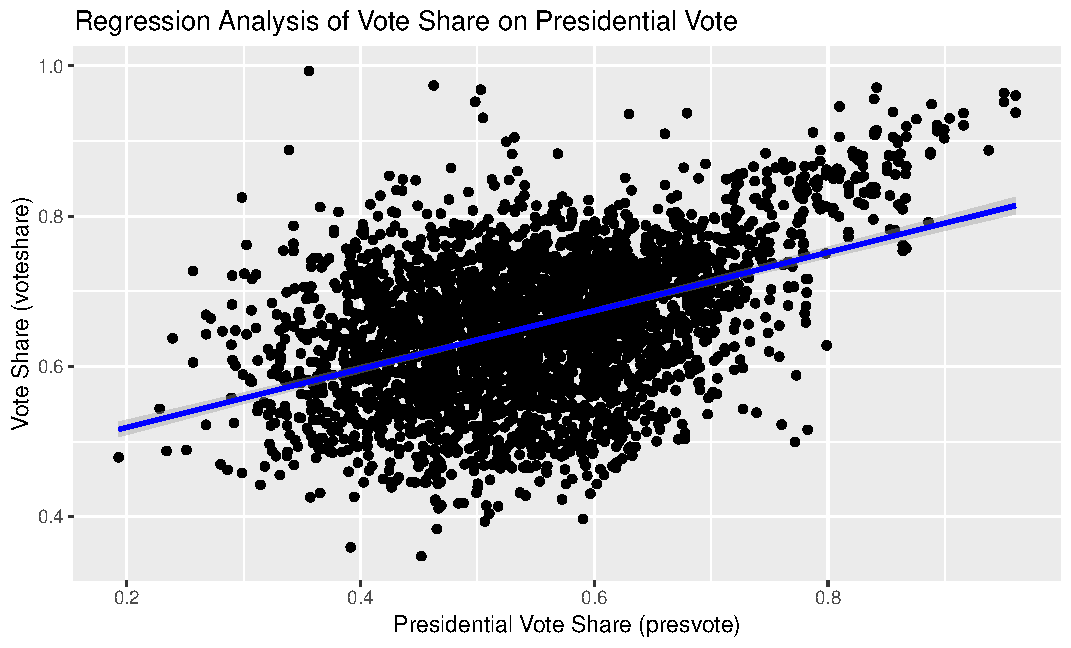
\includegraphics[width=.65\textwidth]{my_answers_question3.2_plot.pdf}
		\end{enumerate}
		\vspace{5cm}
		\item Write the prediction equation.
		\lstinputlisting[language=R, firstline=80, lastline=83]{my_answers_RJ.C.R}
		\begin{verbatim}
			the prediction equation:
			voteshare = 0.441329881204297  +  0.38801844338744 * presvote
		\end{verbatim}
	\end{enumerate}
	

\newpage	
\section*{Question 4}
\noindent The residuals from part (a) tell us how much of the variation in \texttt{voteshare} is $not$ explained by the difference in spending between incumbent and challenger. The residuals in part (b) tell us how much of the variation in \texttt{presvote} is $not$ explained by the difference in spending between incumbent and challenger in the district.
	\begin{enumerate}
		\item Run a regression where the outcome variable is the residuals from Question 1 and the explanatory variable is the residuals from Question 2.	
		\lstinputlisting[language=R, firstline=88, lastline=89]{my_answers_RJ.C.R}
		\begin{verbatim}
			Call:
			lm(formula = residuals ~ residuals_presvote, data = df)
			
			Residuals:
			  Min       1Q     Median      3Q      Max 
			-0.25928 -0.04737 -0.00121  0.04618  0.33126 
			
			Coefficients:
			                   Estimate Std. Error       t value  Pr(>|t|)    
			(Intercept)        -5.934e-18    1.299e-03    0.00        1    
			residuals_presvote  2.569e-01    1.176e-02    21.84   <2e-16 ***
			---
			Signif. codes:  0 ‘***’ 0.001 ‘**’ 0.01 ‘*’ 0.05 ‘.’ 0.1 ‘ ’ 1
			
			Residual standard error: 0.07338 on 3191 degrees of freedom
			Multiple R-squared:   0.13,	Adjusted R-squared:  0.1298 
			F-statistic:   477 on 1 and 3191 DF,  p-value: < 2.2e-16
		\end{verbatim}
		\begin{verbatim}
			Data analysis:
			Residual analysis shows that the minimum residual is -0.25928, 
			the first quartile is -0.04737, the median is -0.00121, the third 
			and fourth quartiles are 0.04618, and the maximum residual is 
			0.33126. This indicates that the residuals are distributed within 
			a certain range and there are no obvious outliers. The intercept 
			is -5.934e-18, the standard error is 1.299e-3, the t-value is 
			0.00, and the p-value is 1. This means that the intercept is not 
			statistically significant and can be considered close to 0.
			The slope is 0.2569, the standard error is 1.176e-2, the t-value 
			is 21.84, and the p-value is less than 2.2e-16. This indicates a 
			significant positive correlation between residuals_redisvote and 
			residues.
			The residual standard error is 0.07338, based on 3191 degrees of 
			freedom. The coefficient of determination is 0.13, and the 
			adjusted coefficient of determination is 0.1298. This indicates 
			that residuals_redisvote can explain approximately 13% of the 
			variance in residuals. F-statistic: 477, based on 1 model degree 
			of freedom and 3191 error degrees of freedom, p-value less than 
			2.2e-16. This indicates that the overall model is statistically 
			significant.
			
			Conclusion:
			For every unit increase in residuals_redisvote, the average 
			increase in residuals is 0.2569 units. The model is statistically 
			significant and explains approximately 13% of the variance in 
			residuals, indicating that resitus_presvote is a useful variable 
			for predicting residuals. These results indicate a significant 
			positive correlation between the residuals of voting shares in 
			presidential elections and those in House of Representatives 
			elections. However, it should be noted that although the 
			correlation is significant, the explanatory power of the model is 
			limited and can only explain a part of the residual variation. 
			This indicates that there are other factors also affecting the 
			residuals.
		\end{verbatim}
		\vspace{0cm}
		\item Make a scatterplot of the two residuals and add the regression line. 	
		\lstinputlisting[language=R, firstline=90, lastline=95]{my_answers_RJ.C.R}
		\begin{enumerate}
			\item[]
			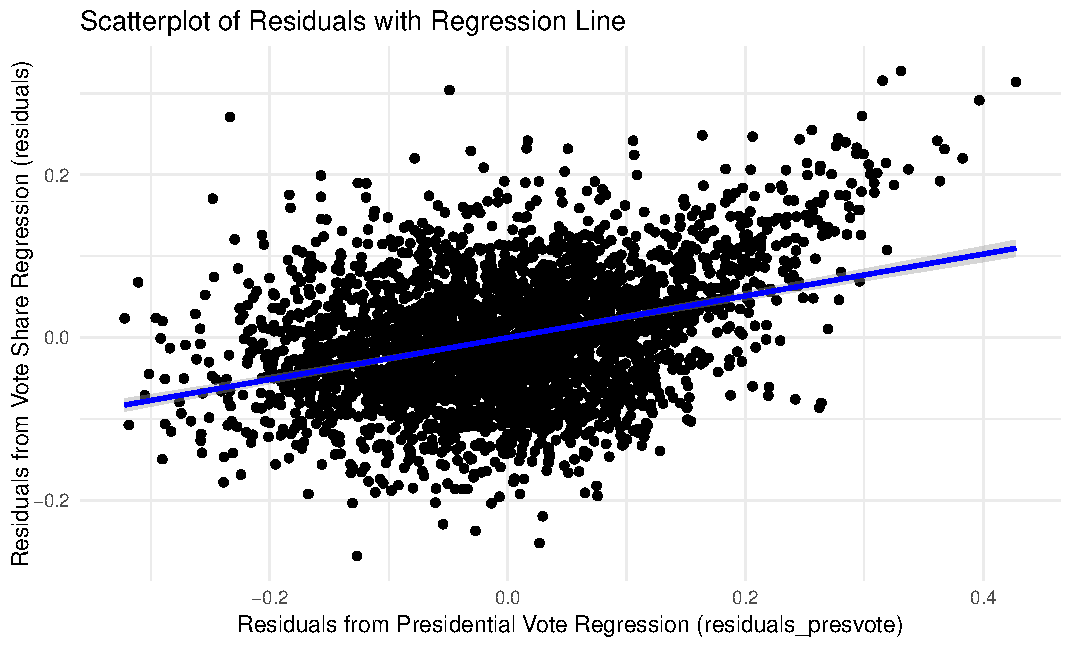
\includegraphics[width=.80\textwidth]{my_answers_question4.2_plot.pdf}
		\end{enumerate}
		\vspace{1cm}
		\item Write the prediction equation.
		\lstinputlisting[language=R, firstline=96, lastline=99]{my_answers_RJ.C.R}
		\begin{verbatim}
			the prediction equation:
			residuals = -5.93407792400741e-18  +  0.256877012700097  * residuals_presvote
		\end{verbatim}
	\end{enumerate}
	
	\newpage	

\section*{Question 5}
\noindent What if the incumbent's vote share is affected by both the president's popularity and the difference in spending between incumbent and challenger? 
	\begin{enumerate}
		\item Run a regression where the outcome variable is the incumbent's \texttt{voteshare} and the explanatory variables are \texttt{difflog} and \texttt{presvote}.	
		\lstinputlisting[language=R, firstline=102, lastline=103]{my_answers_RJ.C.R}
		\begin{verbatim}
			Call:
			lm(formula = voteshare ~ difflog + presvote, data = df)
			
			Residuals:
			  Min       1Q      Median     3Q      Max 
			-0.25928 -0.04737 -0.00121  0.04618  0.33126 
			
			Coefficients:
			          Estimate Std. Error       t value  Pr(>|t|)    
			(Intercept) 0.4486442   0.0063297   70.88   <2e-16 ***
			difflog     0.0355431   0.0009455   37.59   <2e-16 ***
			presvote    0.2568770   0.0117637   21.84   <2e-16 ***
			---
			Signif. codes:  0 ‘***’ 0.001 ‘**’ 0.01 ‘*’ 0.05 ‘.’ 0.1 ‘ ’ 1
			
			Residual standard error: 0.07339 on 3190 degrees of freedom
			Multiple R-squared:  0.4496,	Adjusted R-squared:  0.4493 
			F-statistic:  1303 on 2 and 3190 DF,  p-value: < 2.2e-16
		\end{verbatim}
		\begin{verbatim}
			Data analysis:
			The minimum value is -0.25928. The first quartile is -0.04737. 
			The median is -0.00121. The third and fourth percentiles are 
			0.04618. The maximum value is 0.33126. According to the residual 
			distribution, most residual values are close to 0, indicating 
			that the model fits properly. The distribution range of residuals 
			is from -0.25928 to 0.33126, which is reasonable.
			The intercept is 0.4486442. The coefficient of difflog is 
			0.0355431. The coefficient of presvote is 0.2568770. There are 
			standard errors, t-values, and p-values next to the estimated 
			values of each coefficient. All coefficients have p-values less 
			than 2e-16, which means they are statistically significant.
			The residual standard error is 0.07339. The degree of freedom is 
			3190. The coefficient of determination is 0.4496. The adjusted 
			coefficient of determination is 0.4493. The F-statistic is 1303. 
			The degrees of freedom of the F-statistic are 2 and 3190. The 
			p-value of the F-statistic<2.2e-16 indicates that the model 
			explains 44.96% of the dependent variable variability. The 
			adjusted coefficient of determination takes into account the 
			number of independent variables in the model and slightly 
			decreases to 44.93%. The F-statistic and its p-value indicate 
			that the model as a whole is significant.
			
			Conclusion:
			This linear regression model is statistically significant and explains a significant portion of the variability in voting shares. Both difflog and presvote are significant variables for predicting vote share.
		\end{verbatim}
		\vspace{0cm}
		\item Write the prediction equation.	
		\lstinputlisting[language=R, firstline=104, lastline=110]{my_answers_RJ.C.R}
		\begin{verbatim}
			the prediction equation:
			voteshare = 0.448644221823622  + 0.0355430864025444 * difflog  
			            + 0.256877012700097 * presvote
		\end{verbatim}
		\vspace{0cm}
		\item What is it in this output that is identical to the output in Question 4? Why do you think this is the case?
		\begin{verbatim}
			Similarities
			(1) Residual: The residual statistical data of the two outputs 
			are exactly the same: minimum value: -0.25928, first quartile: 
			-0.04737, median: -0.00121, third and fourth quartiles: 0.04618, 
			maximum value: 0.33126.
			(2) Residual standard error: The residual standard errors of the 
			two outputs are very close, with the fifth output being 0.07339 
			and the fourth output being 0.07338.
			(3) F-statistic and its p-value: The F-statistic and its p-value 
			of both outputs indicate that the model is significant overall, 
			although the specific F-statistic values are different.
			
			Reasons:
			(1) Same dataset or subset: using the same dataset and subset of 
			data. This means that they may have similar residual 
			distributions, resulting in identical residual statistical data.
			(2) May have similar error structures, with error terms following 
			similar distributions in both models.
			(3) Same sample size: If the same number of observations are 
			used, their degrees of freedom will be very close (one is 3190, 
			the other is 3191), resulting in very close residual standard 
			errors
			(4) The significance of the models: The F-statistic and p-value 
			of both models indicate that the models are statistically 
			significant, indicating that both models can effectively explain 
			the variability of the dependent variable.
			(5) The linear relationship of the model: Although the specific 
			variables of the model are different, both models may capture the 
			linear relationship between the independent and dependent 
			variables, which may lead to similarity in the residual 
			distribution.
			(6) The fit of the model: Although the fit of the two models is 
			different, both indicate that the models can explain a certain 
			proportion of data variability.
			(7) Random error: In large sample situations, even if the models 
			are different, random error may produce similar residual patterns
		\end{verbatim}
	\end{enumerate}

\end{document}
